% generated by report/ir2_tables.py, do not edit
\begin{table}[t]
\caption{Idea 1: building the donor layout. Host is the IR1 NumPy/SciPy code on one core, GPU is the same arrays built with CuPy and cuSPARSE (median of 5, synchronised, large from run 3). Identical: all four arrays equal the host ones bit for bit.}
\label{tab:layout}
\small
\begin{tabular}{@{}lrrrc@{}}
\toprule
Size (nnz) & Host ms & GPU ms & Speedup & Identical \\
\midrule
small (3.2 M) & 111.7 & 8.86 & 13$\times$ & yes \\
medium (16.0 M) & 657.0 & 43.02 & 15$\times$ & yes \\
large (76.8 M) & 2,636.9 & 194.42 & 14$\times$ & yes \\
\bottomrule
\end{tabular}
\end{table}

\begin{table*}[t]
\caption{Kernel time in ms (CUDA events, median of 3 trials of 10, or 8 trials for large from run 3, includes the row normalisation) and speedup over the IR1 gather kernel. Max relative error is against the float64 reference after normalisation. 128-thread blocks.}
\label{tab:kernels}
\small
\begin{tabular}{@{}lrrrrrrr@{}}
\toprule
Kernel & \multicolumn{2}{c}{small (3.2 M nnz)} & \multicolumn{2}{c}{medium (16.0 M nnz)} & \multicolumn{2}{c}{large (76.8 M nnz)} & Max rel.\ err \\
 & ms & vs gather & ms & vs gather & ms & vs gather & \\
\midrule
scatter (IR1 v1) & 3.08 & 0.23$\times$ & 25.08 & 0.07$\times$ & 242.4 & 0.02$\times$ & 1.2e-06 \\
gather (IR1 v2) & 0.71 & 1.00$\times$ & 1.72 & 1.00$\times$ & 5.96 & 1.00$\times$ & 2.2e-07 \\
gather\_xr (3b) & 0.42 & 1.68$\times$ & 1.31 & 1.32$\times$ & 6.70 & 0.89$\times$ & 2.2e-07 \\
gather\_fm (3) & 0.39 & 1.84$\times$ & 1.22 & 1.42$\times$ & 4.91 & 1.21$\times$ & 2.2e-07 \\
gather\_cs (2) & 0.82 & 0.87$\times$ & 3.37 & 0.51$\times$ & 10.37 & 0.58$\times$ & 1.2e-06 \\
cuSPARSE SpGEMM & 81.06 & 0.01$\times$ & 323.9 & 0.01$\times$ & -- & -- & 2.8e-07 \\
\bottomrule
\end{tabular}
\end{table*}

\begin{table}[t]
\caption{Idea 2, counted on the host from the actual layouts: adds per nonzero, and lane steps per warp loop iteration (the warp waits for its slowest lane).}
\label{tab:work}
\small
\begin{tabular}{@{}lrrr@{}}
\toprule
 & small & medium & large \\
\midrule
Set bits per cell (no flip) & 19.1 & 19.5 & 19.7 \\
Set bits after the flip & 9.07 & 8.72 & 8.66 \\
Flipped pseudo-bulks (of 900) & 648 & 643 & 645 \\
Adds per nonzero, gather & 32 & 32 & 32 \\
Adds per nonzero, gather\_cs & 10.07 & 9.72 & 9.66 \\
Warp-max set bits per step & 13.84 & 13.46 & 13.56 \\
Lane-step ratio gather / cs & 2.16$\times$ & 2.21$\times$ & 2.20$\times$ \\
\bottomrule
\end{tabular}
\end{table}

\begin{table}[t]
\caption{End to end on the medium instance, ms (median of 5). Host prep is the IR1 layout build or, for the GPU paths, the donor codes. GPU layout includes the fused-mask gather.}
\label{tab:e2e-medium}
\small
\begin{tabular}{@{}lrrrrrr@{}}
\toprule
Path & Host & H2D & Layout & Kernel & D2H & Total \\
\midrule
scatter & 0.0 & 31.6 & 0.0 & 25.3 & 3.6 & \textbf{61.6} \\
gather, host layout (IR1) & 631.7 & 31.9 & 0.0 & 3.2 & 3.3 & \textbf{669.9} \\
gather, GPU layout & 30.9 & 56.1 & 37.8 & 1.7 & 3.3 & \textbf{129.4} \\
gather\_fm, GPU layout & 32.1 & 57.0 & 37.5 & 1.1 & 3.4 & \textbf{130.0} \\
\bottomrule
\end{tabular}
\end{table}

\begin{table}[t]
\caption{End to end on the large instance, ms (median of 5). Host prep is the IR1 layout build or, for the GPU paths, the donor codes. GPU layout includes the fused-mask gather.}
\label{tab:e2e-large}
\small
\begin{tabular}{@{}lrrrrrr@{}}
\toprule
Path & Host & H2D & Layout & Kernel & D2H & Total \\
\midrule
scatter & 0.0 & 147.5 & 0.0 & 242.8 & 6.7 & \textbf{397.1} \\
gather, host layout (IR1) & 2,415.8 & 149.0 & 0.0 & 8.1 & 6.9 & \textbf{2,580.1} \\
gather, GPU layout & 90.4 & 271.1 & 195.2 & 4.8 & 6.8 & \textbf{570.1} \\
gather\_fm, GPU layout & 85.3 & 273.1 & 197.9 & 4.3 & 6.5 & \textbf{566.9} \\
\bottomrule
\end{tabular}
\end{table}

\begin{table}[t]
\caption{Nsight Compute, medium instance, one launch each (SM clock locked at 585 MHz by Nsight, so durations exceed the event timings).}
\label{tab:ncu2}
\footnotesize
\setlength{\tabcolsep}{3pt}
\begin{tabular}{@{}lrrrr@{}}
\toprule
Metric & gather & gather\_xr & gather\_fm & gather\_cs \\
\midrule
Duration (us) & 2,726 & 1,454 & 1,135 & 4,712 \\
SM throughput (\%) & 76.1 & 57.4 & 72.6 & 44.4 \\
L1/TEX throughput (\%) & 86.0 & 74.7 & 69.7 & 89.3 \\
DRAM throughput (\%) & 29.9 & 55.4 & 69.5 & 17.2 \\
Instructions (M) & 160.7 & 79.9 & 78.7 & 110.1 \\
Active threads per instr. & 22.4 & 29.7 & 29.7 & 21.0 \\
Warp cycles per issue & 10.9 & 10.9 & 8.6 & 11.0 \\
Registers per thread & 65 & 65 & 65 & 23 \\
Achieved occupancy (\%) & 84.0 & 79.1 & 79.2 & 33.8 \\
Shared bank conflicts (M) & 0.00 & 0.00 & 0.00 & 21.59 \\
L1/TEX bytes (MB) & 656 & 666 & 269 & 272 \\
DRAM bytes read (MB) & 241 & 238 & 232 & 240 \\
\bottomrule
\end{tabular}
\end{table}

\begin{table}[t]
\caption{Nsight Compute, large (run 3) instance, one launch each (SM clock locked at 585 MHz by Nsight, so durations exceed the event timings).}
\label{tab:ncu-large}
\footnotesize
\setlength{\tabcolsep}{3pt}
\begin{tabular}{@{}lrrrr@{}}
\toprule
Metric & gather & gather\_xr & gather\_fm & gather\_cs \\
\midrule
Duration (us) & 7,494 & 5,391 & 4,106 & 19,170 \\
SM throughput (\%) & 63.8 & 56.6 & 73.1 & 40.6 \\
L1/TEX throughput (\%) & 77.8 & 63.6 & 47.4 & 89.5 \\
DRAM throughput (\%) & 45.5 & 63.2 & 82.2 & 17.8 \\
Instructions (M) & 447.0 & 285.5 & 280.2 & 442.2 \\
Active threads per instr. & 25.1 & 30.7 & 30.7 & 20.6 \\
Warp cycles per issue & 10.5 & 11.5 & 8.9 & 11.2 \\
Registers per thread & 65 & 65 & 65 & 23 \\
Achieved occupancy (\%) & 84.1 & 81.7 & 81.7 & 34.5 \\
Shared bank conflicts (M) & 0.00 & 0.00 & 0.00 & 101.36 \\
L1/TEX bytes (MB) & 2,830 & 2,862 & 914 & 911 \\
DRAM bytes read (MB) & 1,053 & 1,053 & 1,039 & 1,054 \\
\bottomrule
\end{tabular}
\end{table}

\begin{figure}[t]
\centering
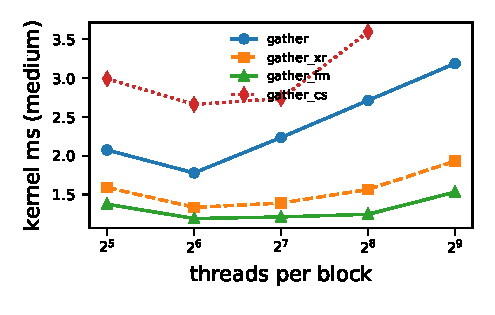
\includegraphics[width=\columnwidth]{figures/ir2_blocks.pdf}
\caption{Block-size sweep on the medium instance (median of 10). gather\_cs stops at 256 threads, where its shared memory reaches 33 KB per block.}
\label{fig:blocks}
\end{figure}

